\chapter{Basic Concepts}

A task can be seen as a sequence of actions and a deadline must be associated to each one of them.\\
We, therefore, are after is a definition of a formal model that identifies what these tasks or actions are and associate deadlines with them.

\section{Real-Time Tasks}
\define{Real-Time Task ($\tau_i$)}{stream of jobs (or instances) $J_{i,k}$, or, in other terms, a sequence of activities that is activated periodically or aperiodically}

Each job $J_{i,k} =  (r_{i,k}, c_{i,k}, d_{i,k})$ is characterised by the following quantities:
\begin{itemize}
    \item{\makebox[1cm]{$r_{i,k}$\hfill}activation time}\pside{activation time}\\
    It is the time at which a task becomes ready for execution; it is also referred as \textit{request time} or \textit{release time}. 
    \item{\makebox[1cm]{$c_{i,k}$\hfill}computation time}\pside{computation time}\\
    Time necessary to the processor for executing the job without interruption.
    \item{\makebox[1cm]{$d_{i,k}$\hfill}absolute deadline}\pside{absolute deadline}\\
    time before which a job should be completed to avoid damage to the system.
    \item{\makebox[1cm]{$f_{i,k}$\hfill}finishing time}\pside{finishing time}\\
    The time at which a job finishes its execution
    \item{\makebox[1cm]{$\rho_{i,k}$\hfill}response time}\pside{response time}\\
    The time at which a job finishes its execution. Formally this quantity is the difference between the finishing time and the activation time.
    \[\rho_{i,k}  = f_{i,k} - r_{i,k}\]
\end{itemize}
Furthermore, since each task $i$ is a sequence of jobs, we need to differentiate between them. That is why each job $J_{i,k}$ is uniquely identified by its task index $i$ and the $k$-th activation of the $i$-th task.\\
In addition, we will say that job $J_{i,k}$ respects its deadline if $f_{i,k} \le d_{i,k}$.



\begin{figure}[!ht]
    \centering
    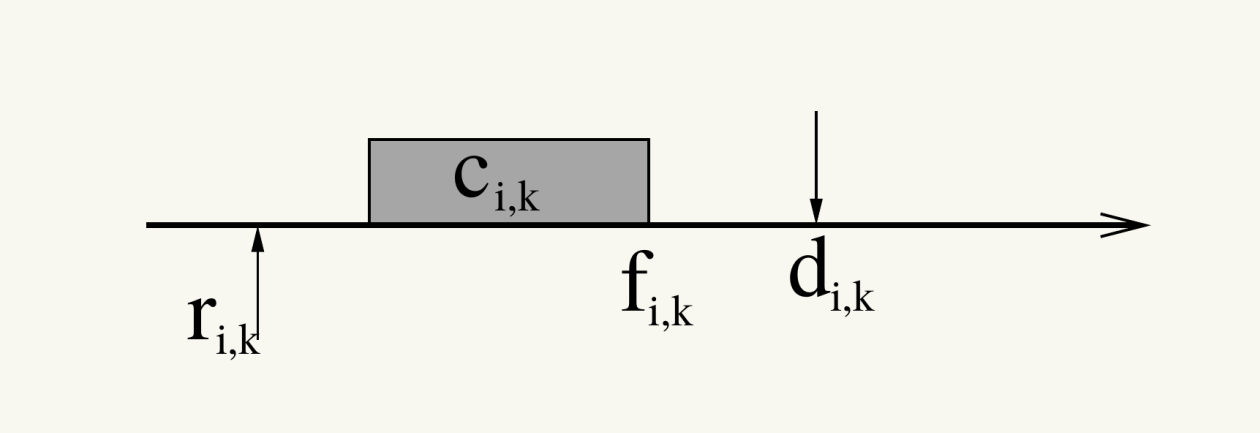
\includegraphics[width = 0.8\textwidth]{images/image01.png}
    \caption{Graphical representation of Mathematical model of a Task}
    \label{fig:image01}
\end{figure}

This mathematical definition of a job in a real-time task holds regardless of the nature of the task itself. In fact, we can identify three different types of tasks: Periodic tasks, Aperiodic Tasks and Sporadic Tasks.
Each of them holds different properties and a different mathematical representation.

\subsection{Periodic Tasks}

\define{Periodic Task}{A periodic task $\tau_i = (C_i, D_i, T_i)$ is a stream of jobs $J_{i,k}$, with:
\begin{align*}
r_{i,k+1} &= r_{i,k} + T_i\\
d_{i,k} &= r_{i,k} + D_i\\
C_i &= \max_k\{c_{i,k}\}
\end{align*}
}
where:
\begin{itemize}
    \item{\makebox[1cm]{$T_i$\hfill}\textbf{Period}}\pside{Period}
    \item{\makebox[1cm]{$D_i$\hfill}\textbf{Relative Deadline}}\pside{Relative Deadline}
    \item{\makebox[1cm]{$C_i$\hfill}\textbf{Worst-Case Execution Time (WCET)}}\pside{Worst-Case Execution Time (WCET)}
    \item{\makebox[1cm]{$R_i$\hfill}\textbf{Worst-Case Response Time (WCRT)}}\pside{Worst-Case Response Time (WCRT)}
    \[R_i = \max_k \{\rho_{i,k}\}=\max_k \{f_{i,k} - r_{i,k}\}\]
\end{itemize}
For the task to be correctly scheduled, it must be $R_i \le D_i$

A periodic task has a regular structure (called \side{cycle}), in the sense that:
\begin{itemize}
\item it is activated periodically with a period of $T_i$
\item it executes a computation
\item when the computation terminates, it suspends waiting for the next period
\end{itemize}

Hence, its fundamental implementation can be represented as:
\begin{lstlisting}[language=C++]
void *PeriodicTask(void *arg)
{
	<initialization>;
	<start periodic timer, period = T>;
	while (condition)
	{
		<read sensors>;
		<update outputs>;
		<update state variables>;
		<wait next activation>;
	}
}
\end{lstlisting}

\subsection{Aperiodic Tasks}

\define{Aperiodic Task}{Aperiodic tasks are not characterised by periodic arrivals, meaning that:
\begin{itemize}
    \item A minimum interarrival time between activations does not exist
    \item Sometimes, aperiodic tasks do not have a particular structure
\end{itemize}
}

Aperiodic tasks can model tasks responding to events that occur rarely (e.g. a mode change) or tasks responding to events with irregular structure (e.g. bursts of packets from the network,\dots).

\subsection{Sporadic Tasks}
Sporadic tasks are aperiodic tasks characterised by a \textbf{Minimum Interarrival Time (MIT)} between jobs.
In this sense they are similar to periodi tasks, but while a periodic task is activated by a periodic timer, a sporadic task is activated by an external event. (e.g. the arrival of a packet from the network)

Hence, its fundamental implementation can be represented as:
\begin{lstlisting}[language=C++]
    void *SporadicTask(void *arg)
    {
        <initialization>;
        while (condition)
        {
            <computation>;
            <wait events>;
        }
    }
\end{lstlisting}
Formally: 
\define{Sporadic Task}{A sporadic task $\tau_i = (C_i, D_i, T_i)$ is a stream of jobs $J_{i,k}$, with:
\begin{align*}
    r_{i,k+1} &\ge r_{i,k} + T_i\\
    d_{i,k+1} &= r_{i,k} + D_i\\
    C_i &= \max_k\{c_{i,k}\}
\end{align*}
}
where:
\begin{itemize}
    \item{\makebox[1cm]{$T_i$\hfill}\textbf{Minimum Interarrival Time (MIT)}}\pside{Minimum Interarrival Time (MIT)}
    \item{\makebox[1cm]{$D_i$\hfill}\textbf{Relative Deadline}}\pside{Relative Deadline}
    \item{\makebox[1cm]{$C_i$\hfill}\textbf{Worst-Case Execution Time (WCET)}}\pside{Worst-Case Execution Time (WCET)}
    \item{\makebox[1cm]{$R_i$\hfill}\textbf{Worst-Case Response Time (WCRT)}}\pside{Worst-Case Response Time (WCRT)}
    \[R_i = \max_k \{\rho_{i,k}\}=\max_k \{f_{i,k} - r_{i,k}\}\]
\end{itemize}
For the task to be correctly scheduled, it must be $R_i \le D_i$.

\section{Task Criticality}
% types of task constraints
A deadline is said to be \textit{hard} if a deadline miss causes a critical failure in the system, whereas a task is said to be a \side{hard real-time task} if all its deadlines are hard, which means that all the deadlines must be guaranteed before starting the task, i.e.
\[\forall j, \rho_{i,j} \le D_i \qquad\Rightarrow\qquad R_i \le D_i\]



\eg{Hard Real-Time Task}{The controller of a mobile robot, must detect obstacles and react within a time dependent on the robot speed, otherwise the robot will crash into the obstacles}

A deadline is said to be \textit{soft} if a deadlien miss causes a degradation in the \side{Quality of Service (QoS)}, but is not a catastrophic event, whereas a task is said to be a \side{soft real-time task} if it has soft deadlines.\\
In other terms, some deadlines can be missed without compromising the correctess of the system, but the number of missed deadlines must be kept under control, because the \textit{quality} of the results depend on the number of missed deadlines.

Unline the hard real-time task, soft real-time tasks can be difficult to characterize, particularly:
\begin{itemize}
\item What's the tradeoff between \textit{non compromising the system correctness} and \textit{not considering missed deadlines}?
\item Moreover, some way to express the QoS experienced by a soft real-time task is needed
\end{itemize}

Examples of QoS definitions could be
\begin{itemize}
\item no more than X consecutive deadlines can be missed
\item no more that X deadlines in an interval of time $T$ can be missed
\item the \side{deadline miss probability} must be less than a specified value, i.e.
\[P\{f_{i,j} > d_{i,j}\} \le R_{max}\]
\item the \side{deadline miss ratio} must be less than a specified value, i.e.
\[\cfrac{\text{number of missed deadlines}}{\text{total number of deadlines}} \le R_{max}\]
\item the maximum \side{tardiness} must be less than a specified value, i.e.
\[\cfrac{R_i}{D_i} < L\]
\item ...
\end{itemize}


\eg{Audio and Video players}{Assuming a framerate of 25 fps, which imply a frame period of 40 ms, if a frame is played a little bit too late, the user might even be unable to notice any degration in the QoS, however, skipped frames can be disturbing.\\
In fact missing a lot of frames by 5 ms can be better than missing only a few frames by 40 ms.}
\eg{Robotic Systems}{Some actuations can be delayed with little consequences on the control quality.}

In any case, soft real-time constraints does not mean no guarantee on dealines, given that tasks can have variable execution times between different jobs.\\
These execution times might depend on different factors:
\begin{itemize}
\item Input data
\item HW issues (cache effects, pipeline stalls, ...)
\item The internal state of the task
\item ...
\end{itemize}

\section{Schedulability analysis}

\subsection{Worst-Case Response Time Analysis}
% can compute an exact result
% any priority assignment and preemptive scheduling

\subsection{Processor Demand Analysis}

\subsection{Processor Utilization Factor test}
% sufficient but not necessary
% does not compute an exact result
% RM assignment and preemptive scheduling